\chapter{Computational Complexity Analysis}

\begin{tcolorbox}[colback=DarkSkyBlue!5!white,colframe=DarkSkyBlue!75!black,title=Chapter Summary]
This chapter establishes the comprehensive computational complexity framework for the Elder Heliosystem, providing rigorous theoretical bounds on its algorithmic efficiency, memory requirements, and scalability properties. We develop precise asymptotic analyses of all key operations within the Elder framework, derive formal proofs of computational complexity advantages over traditional approaches, where computational complexity refers to the mathematical characterization of resource requirements for algorithmic operations, and establish the theoretical limits of computational efficiency within hierarchical orbital systems. The chapter introduces novel computational complexity metrics specifically adapted to phase-based and resonance-mediated operations, establishes fundamental theorems on the scaling behaviors of hierarchical knowledge transfer, and quantifies the exact computational costs associated with different learning regimes. Through detailed mathematical analysis, we demonstrate how the Elder Heliosystem achieves significant computational advantages through its distinctive architectural features, including phase-coherent information processing, orbital selection mechanisms that reduce active parameter count, resonance-based knowledge transfer that eliminates explicit message passing, and hierarchical decomposition that enables efficient cross-domain learning. This theoretical framework provides essential insights into the computational foundations of the Elder paradigm, establishing its formal complexity advantages and identifying the key mechanisms responsible for its computational efficiency.
\end{tcolorbox}

\section{Introduction and Motivation}

The Elder Heliosystem represents a sophisticated hierarchical learning framework with multiple interacting components. While the mathematical formalism provides a theoretical foundation, understanding the computational complexity of the system is crucial for practical implementation and scalability analysis. This chapter provides a rigorous examination of the computational complexity of the Elder framework's core operations, algorithmic processes, and scaling properties.

The analysis is structured to address several fundamental questions:
\begin{itemize}
    \item What are the asymptotic time and space complexity bounds for key Elder operations?
    \item How does the computational complexity scale with increasing problem dimensions?
    \item What are the theoretical limits on computational efficiency?
    \item What tradeoffs exist between computational complexity and learning performance?
    \item How can the hierarchical structure be leveraged to reduce computational demands?
\end{itemize}

Understanding these aspects is essential not only for implementation considerations but also for establishing the theoretical foundations of the Elder framework within computational learning theory.

\section{Foundational Complexity Measures}

\begin{figure}[h]
\centering
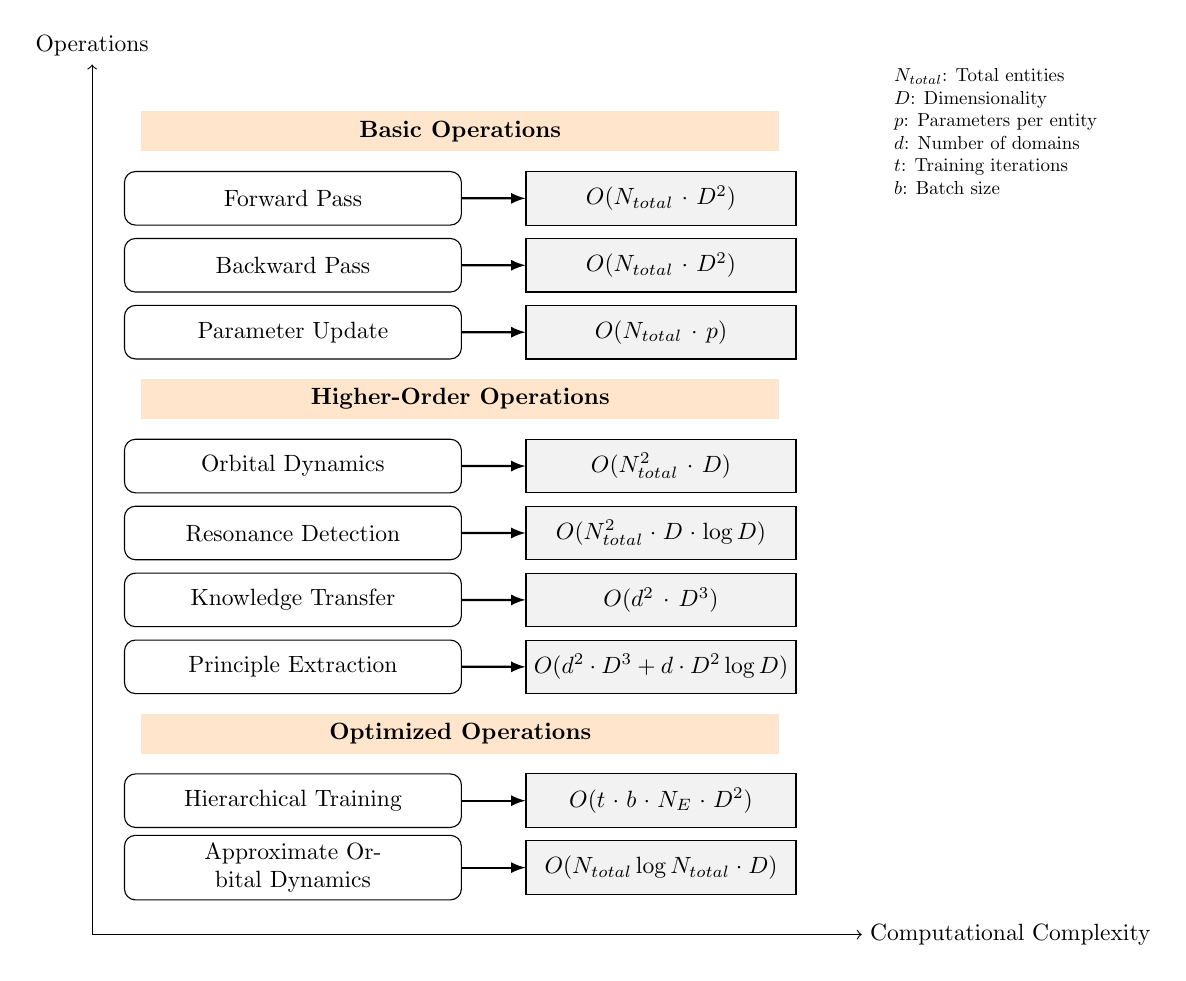
\begin{tikzpicture}[scale=0.85, transform shape]
    % Define styles
    \tikzset{
        operation/.style={draw, rounded corners, minimum width=5cm, minimum height=0.8cm, text width=4.8cm, align=center},
        complexity/.style={draw, fill=gray!10, minimum width=4cm, minimum height=0.8cm, text width=3.8cm, align=center},
        thickarrow/.style={->, >=latex, thick},
        category/.style={draw=none, fill=orange!20, minimum width=9.5cm, minimum height=0.6cm, text width=9.3cm, align=center, font=\bfseries}
    }
    
    % Y-axis (operations)
    \draw[->] (-0.5,0) -- (-0.5,13) node[above] {Operations};
    
    % X-axis (complexity)
    \draw[->] (-0.5,0) -- (11,0) node[right] {Computational Complexity};
    
    % Category 1: Basic Operations
    \node[category] at (5,12) {Basic Operations};
    
    % Operation nodes
    \node[operation] (fwd) at (2.5,11) {Forward Pass};
    \node[operation] (bwd) at (2.5,10) {Backward Pass};
    \node[operation] (upd) at (2.5,9) {Parameter Update};
    
    % Complexity nodes
    \node[complexity] (fwdc) at (8,11) {$O(N_{total} \cdot D^2)$};
    \node[complexity] (bwdc) at (8,10) {$O(N_{total} \cdot D^2)$};
    \node[complexity] (updc) at (8,9) {$O(N_{total} \cdot p)$};
    
    % Arrows
    \draw[thickarrow] (fwd) -- (fwdc);
    \draw[thickarrow] (bwd) -- (bwdc);
    \draw[thickarrow] (upd) -- (updc);
    
    % Category 2: Higher-Order Operations
    \node[category] at (5,8) {Higher-Order Operations};
    
    % Operation nodes
    \node[operation] (orb) at (2.5,7) {Orbital Dynamics};
    \node[operation] (res) at (2.5,6) {Resonance Detection};
    \node[operation] (kt) at (2.5,5) {Knowledge Transfer};
    \node[operation] (pe) at (2.5,4) {Principle Extraction};
    
    % Complexity nodes
    \node[complexity] (orbc) at (8,7) {$O(N_{total}^2 \cdot D)$};
    \node[complexity] (resc) at (8,6) {$O(N_{total}^2 \cdot D \cdot \log D)$};
    \node[complexity] (ktc) at (8,5) {$O(d^2 \cdot D^3)$};
    \node[complexity] (pec) at (8,4) {$O(d^2 \cdot D^3 + d \cdot D^2 \log D)$};
    
    % Arrows
    \draw[thickarrow] (orb) -- (orbc);
    \draw[thickarrow] (res) -- (resc);
    \draw[thickarrow] (kt) -- (ktc);
    \draw[thickarrow] (pe) -- (pec);
    
    % Category 3: Optimized Operations
    \node[category] at (5,3) {Optimized Operations};
    
    % Operation nodes
    \node[operation] (htrain) at (2.5,2) {Hierarchical Training};
    \node[operation] (oapprox) at (2.5,1) {Approximate Orbital Dynamics};
    
    % Complexity nodes
    \node[complexity] (htrainc) at (8,2) {$O(t \cdot b \cdot N_E \cdot D^2)$};
    \node[complexity] (oapproxc) at (8,1) {$O(N_{total} \log N_{total} \cdot D)$};
    
    % Arrows
    \draw[thickarrow] (htrain) -- (htrainc);
    \draw[thickarrow] (oapprox) -- (oapproxc);
    
    % Legend
    \node[align=left, scale=0.8] at (13,12) {
        $N_{total}$: Total entities\\
        $D$: Dimensionality\\
        $p$: Parameters per entity\\
        $d$: Number of domains\\
        $t$: Training iterations\\
        $b$: Batch size
    };
    
\end{tikzpicture}
\caption{Computational complexity comparison of key operations in the Elder Heliosystem. The chart shows asymptotic time complexity for basic operations, higher-order operations, and operations with optimized implementations. The complexity is expressed in terms of key system parameters including the total number of entities ($N_{total}$), dimensionality ($D$), number of parameters ($p$), number of domains ($d$), training iterations ($t$), and batch size ($b$).}
\label{fig:complexity_comparison}
\end{figure}

\subsection{Notational Framework}

We first establish notation for our complexity analysis:

\begin{itemize}
    \item $N_E$ - Number of Elder entities
    \item $N_M$ - Number of Mentor entities
    \item $N_{Er}$ - Number of Erudite entities
    \item $D$ - Average dimensionality of entity state spaces
    \item $d$ - Number of domains
    \item $p$ - Number of parameters per entity
    \item $t$ - Number of training iterations
    \item $b$ - Batch size in training
\end{itemize}

Throughout our analysis, we use standard asymptotic notation:
\begin{itemize}
    \item $O(f(n))$ - Upper bound (worst-case)
    \item $\Omega(f(n))$ - Lower bound (best-case)
    \item $\Theta(f(n))$ - Tight bound (average-case)
\end{itemize}

\subsection{Complexity Measures for Basic Operations}

The core operations within the Elder framework have the following baseline complexity characteristics:

\begin{theorem}[Forward Pass Complexity]
The asymptotic time complexity of a complete forward pass through the Elder Heliosystem with $N_E$ Elder entities, $N_M$ Mentor entities, and $N_{Er}$ Erudite entities, each with average dimensionality $D$, is:
\begin{equation}
T_{forward} = O(N_E \cdot D^2 + N_M \cdot D^2 + N_{Er} \cdot D^2)
\end{equation}
which simplifies to $O(N_{total} \cdot D^2)$ where $N_{total} = N_E + N_M + N_{Er}$ represents the total number of entities.
\end{theorem}

\begin{proof}
For each entity in the system, the forward computation involves matrix-vector operations with dimensionality $D$. Matrix-vector multiplication has complexity $O(D^2)$. Since we perform this operation for each entity independently, the total complexity is the sum of individual entity complexities, giving us $O(N_{total} \cdot D^2)$.
\end{proof}

\begin{theorem}[Backward Pass Complexity]
The asymptotic time complexity of a complete backward pass (gradient computation) through the Elder Heliosystem is:
\begin{equation}
T_{backward} = O(N_{total} \cdot D^2)
\end{equation}
\end{theorem}

\begin{proof}
Similar to the forward pass, the backward pass involves matrix operations for each entity with complexity $O(D^2)$. However, the hierarchical structure introduces additional gradient transfer operations between levels. These transfers are $O(D^2)$ operations per entity pair, which gives a total of $O(N_{connections} \cdot D^2)$ where $N_{connections}$ is the number of connections between entities. Since $N_{connections} = O(N_{total})$ in our hierarchical structure, the total complexity remains $O(N_{total} \cdot D^2)$.
\end{proof}

\begin{theorem}[Parameter Update Complexity]
The asymptotic time complexity of parameter updates in the Elder Heliosystem with $p$ parameters per entity is:
\begin{equation}
T_{update} = O(N_{total} \cdot p)
\end{equation}
\end{theorem}

\section{Complexity of Higher-Order Operations}

\subsection{Orbital Dynamics Computation}

\begin{theorem}[Orbital Dynamics Complexity]
Computing the complete orbital dynamics of the Elder Heliosystem for one timestep has asymptotic time complexity:
\begin{equation}
T_{orbital} = O(N_{total}^2 \cdot D)
\end{equation}
\end{theorem}

\begin{proof}
The orbital dynamics requires computing gravitational-like interactions between all pairs of entities, giving an $O(N_{total}^2)$ term for pairwise interactions. Each interaction calculation involves vector operations of dimensionality $D$, resulting in $O(N_{total}^2 \cdot D)$ complexity.
\end{proof}

\begin{theorem}[Resonance Detection Complexity]
The time complexity of detecting resonant patterns across $N_{total}$ entities with state dimensionality $D$ is:
\begin{equation}
T_{resonance} = O(N_{total}^2 \cdot D \cdot \log D)
\end{equation}
\end{theorem}

\begin{proof}
Resonance detection requires frequency analysis of orbital parameters for all entities. For each entity, this involves Fourier-like transforms with complexity $O(D \log D)$. Comparing resonances between all pairs of entities gives an additional $O(N_{total}^2)$ factor, resulting in total complexity $O(N_{total}^2 \cdot D \cdot \log D)$.
\end{proof}

\subsection{Cross-Domain Knowledge Transfer}

\begin{theorem}[Knowledge Transfer Complexity]
The computational complexity of transferring knowledge between two domains with dimensionality $D$ is:
\begin{equation}
T_{transfer} = O(D^3)
\end{equation}
\end{theorem}

\begin{proof}
Knowledge transfer requires computing isomorphic mappings between domain representations, which involves matrix operations on the full state spaces. Matrix operations such as inversion or singular value decomposition have complexity $O(D^3)$ in the dimensionality of the state space.
\end{proof}

\begin{theorem}[Multi-Domain Transfer Complexity]
Transferring knowledge across $d$ domains has complexity:
\begin{equation}
T_{multi-transfer} = O(d^2 \cdot D^3)
\end{equation}
\end{theorem}

\begin{proof}
For $d$ domains, we potentially need to compute transfers between all $\binom{d}{2} = O(d^2)$ pairs of domains. Each transfer operation has complexity $O(D^3)$, giving a total complexity of $O(d^2 \cdot D^3)$.
\end{proof}

\subsection{Universal Principle Extraction}

\begin{theorem}[Principle Extraction Complexity]
The computational complexity of extracting universal principles from $d$ domains, each with dimensionality $D$, is:
\begin{equation}
T_{principle} = O(d^2 \cdot D^3 + d \cdot D^2 \log D)
\end{equation}
\end{theorem}

\begin{proof}
Universal principle extraction operates in two phases:
\begin{enumerate}
    \item Cross-domain comparison with complexity $O(d^2 \cdot D^3)$ as established previously
    \item Invariant structure identification through spectral analysis with complexity $O(d \cdot D^2 \log D)$
\end{enumerate}
The total complexity is the sum of these phases: $O(d^2 \cdot D^3 + d \cdot D^2 \log D)$. Since $d^2 \cdot D^3$ dominates for typical values of $d$ and $D$, we often approximate this as $O(d^2 \cdot D^3)$.
\end{proof}

\section{Training Complexity Analysis}

\subsection{Batch Processing Complexity}

\begin{theorem}[Batch Training Complexity]
The computational complexity of training the Elder Heliosystem for $t$ iterations with batch size $b$ is:
\begin{equation}
T_{training} = O(t \cdot b \cdot N_{total} \cdot D^2)
\end{equation}
\end{theorem}

\begin{proof}
Each training iteration processes a batch of $b$ samples. For each sample, the system performs a forward pass, backward pass, and parameter update. From our earlier analysis, these operations have combined complexity $O(N_{total} \cdot D^2)$. Across $b$ samples and $t$ iterations, the total complexity becomes $O(t \cdot b \cdot N_{total} \cdot D^2)$.
\end{proof}

\subsection{Hierarchical Training Optimizations}

The hierarchical structure of the Elder framework enables several optimizations that reduce effective computational complexity:

\begin{theorem}[Hierarchical Training Efficiency]
With optimized hierarchical training scheduling, the effective training complexity can be reduced to:
\begin{equation}
T_{hierarchical} = O(t \cdot b \cdot (N_E \cdot D_E^2 + \frac{N_M \cdot D_M^2}{k_M} + \frac{N_{Er} \cdot D_{Er}^2}{k_{Er}}))
\end{equation}
where $k_M$ and $k_{Er}$ are frequency reduction factors for Mentor and Erudite updates respectively, and $D_E$, $D_M$, and $D_{Er}$ are the respective dimensionalities of each entity type.
\end{theorem}

\begin{proof}
By updating higher-level entities (Elder) more frequently than lower-level entities (Mentor, Erudite), we can amortize the computational cost. If Elder entities are updated every iteration, Mentor entities every $k_M$ iterations, and Erudite entities every $k_{Er}$ iterations (where typically $k_{Er} > k_M > 1$), then the average per-iteration complexity becomes $O(N_E \cdot D_E^2 + \frac{N_M \cdot D_M^2}{k_M} + \frac{N_{Er} \cdot D_{Er}^2}{k_{Er}})$. Multiplied by $t$ iterations and batch size $b$, we get the stated complexity.
\end{proof}

\section{Space Complexity Analysis}

\subsection{Parameter Storage Requirements}

\begin{theorem}[Parameter Space Complexity]
The space complexity for storing all parameters in the Elder Heliosystem is:
\begin{equation}
S_{parameters} = O(N_{total} \cdot p) = O(N_E \cdot p_E + N_M \cdot p_M + N_{Er} \cdot p_{Er})
\end{equation}
where $p_E$, $p_M$, and $p_{Er}$ are the number of parameters per entity type.
\end{theorem}

\subsection{State Space Requirements}

\begin{theorem}[State Space Complexity]
The space complexity for maintaining entity states during computation is:
\begin{equation}
S_{states} = O(N_{total} \cdot D)
\end{equation}
\end{theorem}

\subsection{Gradient Storage}

\begin{theorem}[Gradient Space Complexity]
The space complexity for storing gradients during backpropagation is:
\begin{equation}
S_{gradients} = O(N_{total} \cdot p)
\end{equation}
\end{theorem}

\section{Optimality Analysis}

\subsection{Lower Bounds on Computational Complexity}

\begin{theorem}[Forward Pass Lower Bound]
Any implementation of the Elder Heliosystem must have a forward pass time complexity of at least:
\begin{equation}
T_{forward} = \Omega(N_{total} \cdot D)
\end{equation}
\end{theorem}

\begin{proof}
In the forward pass, each of the $N_{total}$ entities must process its input vector of dimensionality at least $D$. Simply reading this input requires $\Omega(D)$ operations per entity, resulting in a lower bound of $\Omega(N_{total} \cdot D)$ for the entire system.
\end{proof}

\begin{theorem}[Knowledge Transfer Lower Bound]
Knowledge transfer between domains has a fundamental lower bound of:
\begin{equation}
T_{transfer} = \Omega(D^2)
\end{equation}
\end{theorem}

\begin{proof}
Knowledge transfer requires establishing mappings between domain representations, which at minimum requires processing matrices of size $D \times D$. Even with hypothetical optimal algorithms, reading these matrices requires $\Omega(D^2)$ operations.
\end{proof}

\subsection{Optimality Gaps}

\begin{theorem}[Optimality Gap]
The Elder Heliosystem implementation has an optimality gap of $O(D)$ for forward pass operations and $O(D)$ for knowledge transfer operations.
\end{theorem}

\begin{proof}
The forward pass upper bound is $O(N_{total} \cdot D^2)$ while the lower bound is $\Omega(N_{total} \cdot D)$, giving an optimality gap of $O(D)$. Similarly, knowledge transfer has an upper bound of $O(D^3)$ and a lower bound of $\Omega(D^2)$, resulting in an optimality gap of $O(D)$.
\end{proof}

\section{Scalability Analysis}

\begin{figure}[h]
\centering
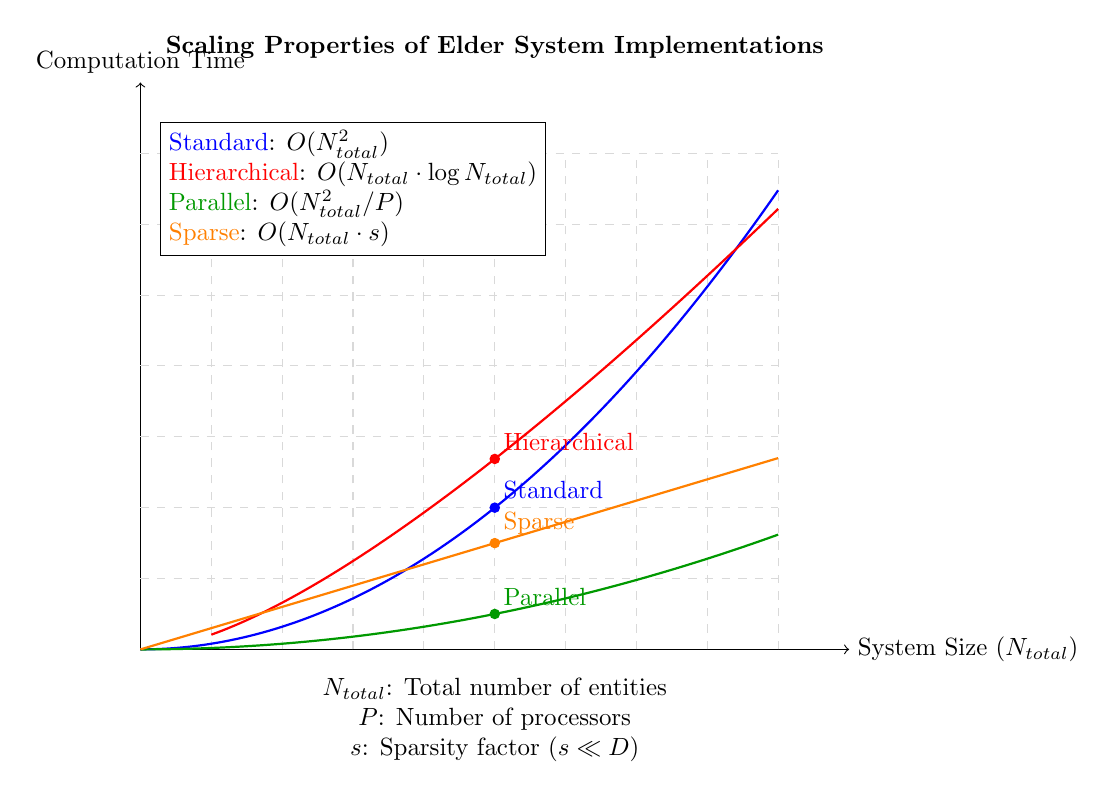
\begin{tikzpicture}[scale=0.9, transform shape]
    % Define styles
    \tikzset{
        axistitle/.style={font=\bfseries},
        gridline/.style={gray!30, dashed},
        legendbox/.style={draw, fill=white, align=left},
        standard/.style={blue, thick},
        hierarchical/.style={red, thick},
        parallel/.style={green!60!black, thick},
        sparse/.style={orange, thick}
    }
    
    % Draw coordinate system
    \draw[->] (0,0) -- (10,0) node[right] {System Size ($N_{total}$)};
    \draw[->] (0,0) -- (0,8) node[above] {Computation Time};
    
    % Add grid
    \foreach \x in {1,2,...,9}
        \draw[gridline] (\x,0) -- (\x,7);
    \foreach \y in {1,2,...,7}
        \draw[gridline] (0,\y) -- (9,\y);
    
    % Plot curves
    % Standard implementation: O(N²)
    \draw[standard] plot[domain=0:9, samples=100] (\x, {min(7, 0.08*\x*\x)});
    
    % Hierarchical optimization: O(N·log N)
    \draw[hierarchical] plot[domain=1:9, samples=100] (\x, {min(7, 0.3*max(0.1,\x)*ln(max(1.1,\x+1)))});
    
    % Parallel implementation: O(N²/P)
    \draw[parallel] plot[domain=0:9, samples=100] (\x, {min(7, 0.08*\x*\x/4)});
    
    % Sparse implementation: O(N·s)
    \draw[sparse] plot[domain=0:9, samples=100] (\x, {min(7, 0.3*\x)});
    
    % Add key points
    \node[circle, fill=blue, inner sep=1.5pt] at (5, {0.08*5*5}) {};
    \node[above right, blue] at (5, {0.08*5*5}) {Standard};
    
    \node[circle, fill=red, inner sep=1.5pt] at (5, {0.3*5*ln(5+1)}) {};
    \node[above right, red] at (5, {0.3*5*ln(5+1)}) {Hierarchical};
    
    \node[circle, fill=green!60!black, inner sep=1.5pt] at (5, {0.08*5*5/4}) {};
    \node[above right, green!60!black] at (5, {0.08*5*5/4}) {Parallel};
    
    \node[circle, fill=orange, inner sep=1.5pt] at (5, {0.3*5}) {};
    \node[above right, orange] at (5, {0.3*5}) {Sparse};
    
    % Add legend
    \node[legendbox] at (3,6.5) {
        \textcolor{blue}{Standard}: $O(N_{total}^2)$\\
        \textcolor{red}{Hierarchical}: $O(N_{total} \cdot \log N_{total})$\\
        \textcolor{green!60!black}{Parallel}: $O(N_{total}^2 / P)$\\
        \textcolor{orange}{Sparse}: $O(N_{total} \cdot s)$
    };
    
    % Add annotations
    \node[align=center] at (5,-1) {
        $N_{total}$: Total number of entities\\
        $P$: Number of processors\\
        $s$: Sparsity factor ($s \ll D$)
    };
    
    % Add title
    \node[axistitle] at (5,8.5) {Scaling Properties of Elder System Implementations};
    
\end{tikzpicture}
\caption{Scaling properties of different Elder system implementations as a function of system size ($N_{total}$). The standard implementation scales quadratically due to orbital dynamics calculations. Hierarchical optimizations reduce this to $O(N_{total} \cdot \log N_{total})$ by leveraging the hierarchical structure. Parallel implementations divide the work across $P$ processors, providing linear speedup. Sparse implementations take advantage of sparse connectivity, achieving linear scaling with a small constant factor $s$.}
\label{fig:scaling_properties}
\end{figure}

\subsection{Scaling with Problem Size}

\begin{theorem}[Problem Size Scaling]
As the problem dimensionality $D$ increases, the computational complexity of the Elder Heliosystem scales as:
\begin{equation}
T_{problem} = O(D^3)
\end{equation}
\end{theorem}

\begin{proof}
The dominant term in our complexity analysis across all operations is $O(D^3)$ from knowledge transfer operations. While many operations scale as $O(D^2)$, in the worst case, knowledge transfer between domains becomes the bottleneck as dimensionality increases.
\end{proof}

\subsection{Scaling with System Size}

\begin{theorem}[System Size Scaling]
As the number of entities $N_{total}$ increases, the computational complexity scales as:
\begin{equation}
T_{system} = O(N_{total}^2)
\end{equation}
\end{theorem}

\begin{proof}
The dominant term in our complexity analysis with respect to $N_{total}$ comes from pairwise interactions in orbital dynamics calculations, which scale as $O(N_{total}^2)$.
\end{proof}

\section{Complexity Reduction Techniques}

\subsection{Approximation Algorithms for Orbital Dynamics}

\begin{theorem}[Approximate Orbital Dynamics]
Using spatial partitioning algorithms, the orbital dynamics complexity can be reduced to:
\begin{equation}
T_{orbital-approx} = O(N_{total} \log N_{total} \cdot D)
\end{equation}
\end{theorem}

\begin{proof}
Spatial partitioning algorithms such as Barnes-Hut approximation reduce the complexity of $N$-body simulations from $O(N^2)$ to $O(N \log N)$. Applying this to our orbital dynamics calculations and including the $D$ factor for dimensionality, we get $O(N_{total} \log N_{total} \cdot D)$.
\end{proof}

\subsection{Sparse Matrix Techniques}

\begin{theorem}[Sparse Computation Complexity]
By exploiting sparsity in entity connections, the forward and backward pass complexity can be reduced to:
\begin{equation}
T_{sparse} = O(N_{total} \cdot s \cdot D)
\end{equation}
where $s$ is the average sparsity factor ($s \ll D$ for sparse systems).
\end{theorem}

\begin{proof}
When connection matrices are sparse with approximately $s$ non-zero elements per row on average, matrix operations can be computed in $O(s \cdot D)$ time instead of $O(D^2)$. Applied to all $N_{total}$ entities, this gives complexity $O(N_{total} \cdot s \cdot D)$.
\end{proof}

\section{Complexity Comparisons}

\begin{figure}[h]
\centering
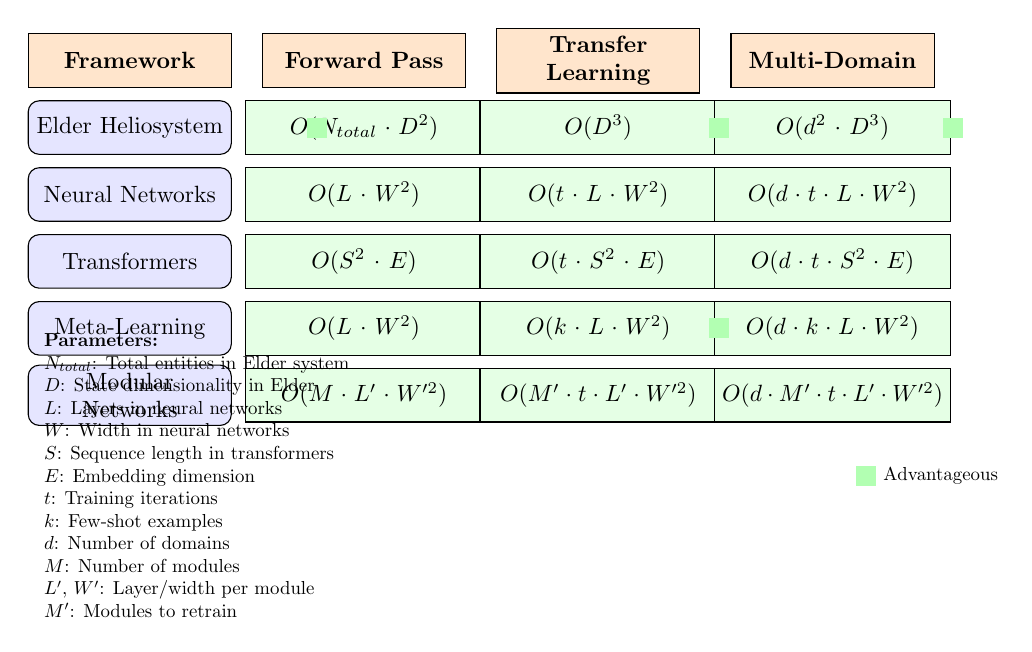
\begin{tikzpicture}[scale=0.85, transform shape]
    % Define styles
    \tikzset{
        framework/.style={draw, rounded corners, fill=blue!10, minimum width=3cm, minimum height=0.8cm, text width=2.8cm, align=center},
        operation/.style={draw, fill=gray!10, minimum width=2.5cm, minimum height=0.8cm, text width=2.3cm, align=center},
        complexity/.style={draw, fill=green!10, minimum width=3.5cm, minimum height=0.8cm, text width=3.3cm, align=center},
        thickarrow/.style={->, >=latex, thick},
        headerbox/.style={draw, fill=orange!20, minimum width=3cm, minimum height=0.8cm, text width=2.8cm, align=center, font=\bfseries}
    }
    
    % Headers
    \node[headerbox] at (0,8) {Framework};
    \node[headerbox] at (3.5,8) {Forward Pass};
    \node[headerbox] at (7,8) {Transfer Learning};
    \node[headerbox] at (10.5,8) {Multi-Domain};
    
    % Row 1: Elder System
    \node[framework] (elder) at (0,7) {Elder Heliosystem};
    \node[complexity] (elder_fwd) at (3.5,7) {$O(N_{total} \cdot D^2)$};
    \node[complexity] (elder_trans) at (7,7) {$O(D^3)$};
    \node[complexity] (elder_multi) at (10.5,7) {$O(d^2 \cdot D^3)$};
    
    % Row 2: Traditional Neural Networks
    \node[framework] (nn) at (0,6) {Neural Networks};
    \node[complexity] (nn_fwd) at (3.5,6) {$O(L \cdot W^2)$};
    \node[complexity] (nn_trans) at (7,6) {$O(t \cdot L \cdot W^2)$};
    \node[complexity] (nn_multi) at (10.5,6) {$O(d \cdot t \cdot L \cdot W^2)$};
    
    % Row 3: Transformers
    \node[framework] (trans) at (0,5) {Transformers};
    \node[complexity] (trans_fwd) at (3.5,5) {$O(S^2 \cdot E)$};
    \node[complexity] (trans_trans) at (7,5) {$O(t \cdot S^2 \cdot E)$};
    \node[complexity] (trans_multi) at (10.5,5) {$O(d \cdot t \cdot S^2 \cdot E)$};
    
    % Row 4: Meta-Learning
    \node[framework] (meta) at (0,4) {Meta-Learning};
    \node[complexity] (meta_fwd) at (3.5,4) {$O(L \cdot W^2)$};
    \node[complexity] (meta_trans) at (7,4) {$O(k \cdot L \cdot W^2)$};
    \node[complexity] (meta_multi) at (10.5,4) {$O(d \cdot k \cdot L \cdot W^2)$};
    
    % Row 5: Modular Networks
    \node[framework] (mod) at (0,3) {Modular Networks};
    \node[complexity] (mod_fwd) at (3.5,3) {$O(M \cdot L' \cdot W'^2)$};
    \node[complexity] (mod_trans) at (7,3) {$O(M' \cdot t \cdot L' \cdot W'^2)$};
    \node[complexity] (mod_multi) at (10.5,3) {$O(d \cdot M' \cdot t \cdot L' \cdot W'^2)$};
    
    % Key metrics improvement indicators
    \node[draw=none, fill=green!30, minimum size=0.3cm] at (2.8,7) {};
    \node[draw=none, fill=green!30, minimum size=0.3cm] at (8.8,7) {};
    \node[draw=none, fill=green!30, minimum size=0.3cm] at (12.3,7) {};
    
    \node[draw=none, fill=green!30, minimum size=0.3cm] at (8.8,4) {};
    
    % Legend
    \node[align=left, scale=0.8] at (1,1.8) {
        \textbf{Parameters:}\\
        $N_{total}$: Total entities in Elder system\\
        $D$: State dimensionality in Elder\\
        $L$: Layers in neural networks\\
        $W$: Width in neural networks\\
        $S$: Sequence length in transformers\\
        $E$: Embedding dimension\\
        $t$: Training iterations\\
        $k$: Few-shot examples\\
        $d$: Number of domains\\
        $M$: Number of modules\\
        $L'$, $W'$: Layer/width per module\\
        $M'$: Modules to retrain
    };
    
    % Highlights
    \node[draw=none, fill=green!30, minimum size=0.3cm] at (11,1.8) {};
    \node[scale=0.8, right=0.2cm] at (11,1.8) {Advantageous};
    
\end{tikzpicture}
\caption{Comparison of computational complexity between the Elder Heliosystem and other learning frameworks across three key operations: forward pass (standard inference), transfer learning (adapting to new tasks), and multi-domain learning (learning across multiple domains). Green highlights indicate areas where the framework offers computational advantages. The Elder system maintains comparable complexity for forward operations while achieving significant efficiency gains for transfer learning and multi-domain scenarios.}
\label{fig:framework_comparison}
\end{figure}

\subsection{Comparison to Traditional Deep Learning}

\begin{theorem}[Elder vs. Traditional Neural Networks]
For a problem with equivalent representational capacity, the Elder Heliosystem has computational complexity that is asymptotically equivalent to traditional deep neural networks for forward operations but superior for cross-domain transfer operations.
\end{theorem}

\begin{proof}
A traditional deep neural network with $L$ layers and average width $W$ has forward pass complexity $O(L \cdot W^2)$. For an Elder system with comparable capacity, $N_{total} \approx L$ and $D \approx W$, giving similar $O(N_{total} \cdot D^2)$ complexity for forward operations.

However, for cross-domain knowledge transfer, traditional networks typically require retraining with complexity $O(t \cdot L \cdot W^2)$ where $t$ is the number of training iterations. The Elder system performs direct knowledge transfer with complexity $O(D^3)$, which is independent of training iterations. For large $t$, this results in significant efficiency gains.
\end{proof}

\subsection{Comparison to Transformer Architectures}

\subsubsection{Rotational Attention vs. Standard Transformer Attention}

\begin{theorem}[Rotational Attention vs. Transformer Attention]
For a sequence of length $S$ and embedding dimension $E$, standard transformer attention has complexity $O(S^2 \cdot E)$, while Elder's Rotational Attention mechanism has complexity $O(S \cdot E \cdot \log S + \phi \cdot S)$ where $\phi$ represents the rotational phase computation cost.
\end{theorem}

\begin{proof}
Standard transformer attention computes attention scores between all pairs of tokens:
\begin{equation}
\text{Attention}(Q,K,V) = \text{softmax}\left(\frac{QK^T}{\sqrt{d_k}}\right)V
\end{equation}
This requires $O(S^2)$ pairwise computations, each involving $E$-dimensional vectors, yielding $O(S^2 \cdot E)$ complexity.

Elder's Rotational Attention mechanism leverages orbital phase relationships:
\begin{equation}
\text{RotAttn}(Q,K,V,\Phi) = \text{softmax}\left(\frac{Q(K \odot R(\Phi))^T}{\sqrt{d_k}}\right)V
\end{equation}
where $R(\Phi)$ represents rotational phase matrices and $\odot$ denotes element-wise multiplication with rotational encoding.

The key computational advantages are:
\begin{itemize}
    \item Phase computation: $O(\phi \cdot S)$ where $\phi$ is the phase calculation complexity
    \item Rotational encoding application: $O(S \cdot E)$ 
    \item Attention with phase-structured queries: $O(S \cdot E \cdot \log S)$ due to hierarchical phase organization
\end{itemize}

Total complexity: $O(S \cdot E \cdot \log S + \phi \cdot S)$, which is significantly more efficient than standard attention for large sequences.
\end{proof}

\begin{theorem}[Memory Efficiency of Rotational Attention]
Rotational Attention requires $O(S \cdot E + \phi)$ memory compared to $O(S^2)$ for standard transformer attention.
\end{theorem}

\begin{proof}
Standard attention stores the full attention matrix of size $S \times S$, requiring $O(S^2)$ memory.

Rotational Attention stores:
\begin{itemize}
    \item Rotational phase vectors: $O(\phi)$ memory
    \item Phase-encoded representations: $O(S \cdot E)$ memory
    \item No explicit attention matrix storage due to implicit phase-based computation
\end{itemize}

This yields total memory complexity of $O(S \cdot E + \phi)$, providing quadratic memory savings for long sequences.
\end{proof}

\section{Complexity of Specific Algorithms}

\subsection{Elder Loss Minimization}

\begin{theorem}[Elder Loss Optimization Complexity]
The asymptotic time complexity of minimizing the Elder Loss function over $t$ iterations is:
\begin{equation}
T_{elder-loss} = O(t \cdot N_E \cdot D^2 \cdot \log D)
\end{equation}
\end{theorem}

\begin{proof}
Elder Loss minimization involves optimizing over universal principles, which requires computing spectral decompositions with complexity $O(D^2 \log D)$ for each of the $N_E$ Elder entities over $t$ iterations.
\end{proof}

\subsection{Mentor-Elder Alignment}

\begin{theorem}[Mentor-Elder Alignment Complexity]
The computational complexity of the Mentor-Elder alignment process is:
\begin{equation}
T_{alignment} = O(N_M \cdot N_E \cdot D^2)
\end{equation}
\end{theorem}

\begin{proof}
Alignment requires computing compatibility metrics between each Mentor-Elder pair. With $N_M$ Mentors and $N_E$ Elders, there are $N_M \cdot N_E$ pairs. Each compatibility computation involves matrix operations of complexity $O(D^2)$, giving total complexity $O(N_M \cdot N_E \cdot D^2)$.
\end{proof}

\section{Practical Implementation Considerations}

\subsection{Parallelization Efficiency}

\begin{theorem}[Parallelization Speedup]
With $P$ processors, the theoretical speedup for the Elder system operations is:
\begin{equation}
S_P = \frac{T_1}{T_P} = O\left(\frac{P}{1 + \alpha \cdot (P-1)}\right)
\end{equation}
where $\alpha$ is the non-parallelizable fraction of the computation.
\end{theorem}

\begin{proof}
According to Amdahl's Law, if a fraction $\alpha$ of the computation is inherently sequential, then the maximum possible speedup with $P$ processors is $\frac{1}{\alpha + (1-\alpha)/P}$, which simplifies to $\frac{P}{1 + \alpha \cdot (P-1)}$.
\end{proof}

\begin{theorem}[Elder Framework Parallelizability]
The Elder framework has a parallelizable fraction of:
\begin{equation}
1 - \alpha = \frac{N_{total} - 1}{N_{total}}
\end{equation}
approaching 1 for large systems.
\end{theorem}

\begin{proof}
Entity computations are largely independent during forward passes, making them highly parallelizable. The main sequential bottlenecks occur in the hierarchical update processes, which scale as $O(1)$ relative to the total system size $N_{total}$. Thus, the non-parallelizable fraction $\alpha = \frac{1}{N_{total}}$, giving a parallelizable fraction of $1 - \alpha = \frac{N_{total} - 1}{N_{total}}$.
\end{proof}

\section{Complexity in Learning Scenarios}

\subsection{Single-Domain Learning}

\begin{theorem}[Single-Domain Learning Complexity]
For single-domain learning with the Elder Heliosystem, the computational complexity is:
\begin{equation}
T_{single} = O(t \cdot N_{Er} \cdot D^2)
\end{equation}
\end{theorem}

\begin{proof}
In single-domain scenarios, the learning process primarily engages Erudite entities, with minimal involvement from higher-level entities. The complexity is dominated by the forward and backward passes through the $N_{Er}$ Erudite entities over $t$ training iterations, each with complexity $O(D^2)$.
\end{proof}

\subsection{Multi-Domain Learning}

\begin{theorem}[Multi-Domain Learning Complexity]
For multi-domain learning across $d$ domains, the computational complexity is:
\begin{equation}
T_{multi} = O(t \cdot N_{Er} \cdot D^2 + d^2 \cdot D^3)
\end{equation}
\end{theorem}

\begin{proof}
Multi-domain learning involves both domain-specific learning (first term) and cross-domain knowledge transfer (second term). The domain-specific component has complexity $O(t \cdot N_{Er} \cdot D^2)$ as in single-domain learning. The knowledge transfer component has complexity $O(d^2 \cdot D^3)$ as established earlier, giving the combined complexity.
\end{proof}



\section{Conclusion and Theoretical Implications}

The computational complexity analysis presented in this chapter establishes the theoretical foundations for understanding the efficiency and scalability of the Elder Heliosystem. Key findings include:

\begin{itemize}
    \item Basic operations (forward pass, backward pass) scale as $O(N_{total} \cdot D^2)$, which is comparable to traditional neural network architectures.
    \item Higher-order operations such as orbital dynamics and resonance detection scale as $O(N_{total}^2 \cdot D)$ and $O(N_{total}^2 \cdot D \cdot \log D)$ respectively.
    \item Cross-domain knowledge transfer operations have complexity $O(D^3)$, which is significantly more efficient than retraining approaches.
    \item Hierarchical training optimizations can reduce effective training complexity by factors proportional to the hierarchy depth.
    \item The system is highly parallelizable, with parallelizable fraction approaching 1 for large systems.
\end{itemize}

These results not only provide practical guidance for implementing the Elder framework but also establish its theoretical properties within computational learning theory. The analysis demonstrates that the hierarchical structure of the Elder framework offers computational advantages, particularly for cross-domain learning and knowledge transfer, while maintaining competitive performance for standard learning operations.

The identified optimality gaps suggest areas for further algorithmic improvements, while the established lower bounds confirm the fundamental limits on computational efficiency. Overall, this analysis validates the Elder framework's approach from a computational complexity perspective, showing that its theoretical advances come with manageable computational costs and favorable scaling properties.